\chapter{Resultat}
\label{chap:resultat}

In der vorliegenden Arbeit wurde eingangs in \fref{chap:engine-uebersicht} aus den gestiegenen Anforderungen an Softwareprojekte in der Spielebranche die Motivation entwickelt, neue Mittel und Wege für das Beherrschen der zunehmenden Komplexität zu suchen. Es wurde festgestellt, dass die Programmiersprache das wichtigste Kommunikationsmittel unter den Softwareentwicklern ist. Dementsprechend spielt die Programmiersprache eine zentrale Rolle in den Softwareprojekten. Sie bestimmt die Kommunikation aber auch die Softwarearchitektur und die Möglichkeiten der Entwickler.

Jede Branche und jedes Projekt besitzt eigene individuelle Anforderungen und Herausforderungen. In der Grafik-Engine-Entwicklung stellen die Grafik-\ac{API}s die Kernherausforderungen. In \fref{chap:modern-opengl} wurde am Beispiel von \textit{OpenGL} die Entwicklung der Grafik-\ac{API} betrachtet und welche Herausforderungen und Möglichkeiten diese Schnittstelle mit sich bringt.

\fref{chap:loesungen-durch-fp} zitierte Entwicklergrößen aus der Spielebranche. Die getroffenen Aussagen geben die aktuellen Probleme in der Spiele- und Engine-Entwicklung wieder. Es wurde gezeigt, dass die wesentlichen Probleme, die sich in den Industriesprachen C++, C\# oder Java zeigen, in anderen Sprachen entweder konzeptionell keine Probleme darstellen oder bereits gelöst sind. Diese Diskussion wird in diesem Kapitel in \fref{sec:xp-haskell} noch einmal abschließend aufgegriffen und um persönliche Einschätzungen des Autors erweitert.

Aus der Motiviation heraus neue Wege und Lösungen für aktuelle Probleme in der Engine-Entwicklung zu suchen, wurde in \fref{chap:ueberblick-pipeline} eine Renderkomponente einer Engine in Haskell entwickelt. Es wurde gezeigt, dass einfache funktionale Konzepte zu einer hohen Komponierbarkeit der einzelen Bausteine mit geringen Reibungsverlusten führt.

Neben der theoretischen Konzeption war ein wesentlicher Teil dieser Arbeit die praktische Anwendung des Konzepts. Es wurde Eingangs das Ziel gesteckt, dass in \fref{chap:pbr} beschriebene \ac{PBR} Konzept, mit der entwickelten Renderkomponente umzusetzen. Die praktische Umsetzung eines aktuellen Echtzeit-Rendering-Verfahrens dient dabei als praktischer Beweis der Machbarkeit und Anwendbarkeit des Konzepts auf konkrete praktische Problemstellungen. Die Implementierung wird in diesem Kapitel in \fref{sec:diskussion-impl} noch einmal genauer beleuchtet.

\section{Diskussion der Implementierung}\label{sec:diskussion-impl}

Im Fokus deser Arbeit stand die Konzeption der Renderkomponente der Engine, wärhend die Detailbetrachtung der einzelnen Renderschritte in den Hintergrund gerückt ist. Exemplarisch wurde in \fref{chap:anwendung} ein einfacher Renderschritt implementiert, um das generelle Vorgehen zu verdeutlichen. Grundlegende Entscheidungen werden in \fref{sec:konzepte-impl} erläutert und begründet. In \fref{sec:laufzeit-impl} wird das Laufzeitverhalten in der Praxis kurz dargestellt und analysiert.

\subsection{Konzepte der Implementierung}\label{sec:konzepte-impl}

Es wurde für die Implementierung der Renderschritte auf eine Abstraktion der Grafik-\ac{API} verzichtet. Zum einen, da ausschließlich \textit{OpenGL} zum Einsatz kommen sollte, und die Abstraktionsschicht nicht benötigt wurde, um die Grafikschnittstelle flexibel austauschen zu können. Zum anderen sollte die Umsetzung möglichst direkt \textit{OpenGL} verwenden. Dies machte es auch einfacher \textit{OpenGL} Beispiele nach Haskell zu übertragen. Der Verzicht auf eine Abstraktionsschicht reduzierte auch den Aufwand für die Umsetzung des Projekt auf ein vertratbares Niveau. Zudem ist der aktuelle Stand von \textit{OpenGL}\footnote{Version 4.3 zum Zeitpunkt der Projektphase} noch schwer mit funktionalen Konzepten einzufangen (siehe: \fref{chap:haskell-modern-gl}).

Die direkte Umsetzung der Logik eines Renderschritts in \textit{OpenGL} vereinfacht zudem die Verwendung von \textit{OpenGL} Erweiterungen. Dies war für die praktische Umsetzung des \ac{PBR} Verfahrens von Bedeutung, da einige spezielle Erweiterungen\footnote{z.B. ARB\_shading\_language\_include : https://www.opengl.org/registry/specs/ARB/shading\_language\_include.txt} verwendet wurden. Auch in der Implementierung von \acf{AO} mittels \textit{Sparse Textures} wurden spezielle Erweiterungen benötigt.

\begin{figure}
\begin{subfigure}{\textwidth}
	\centering
	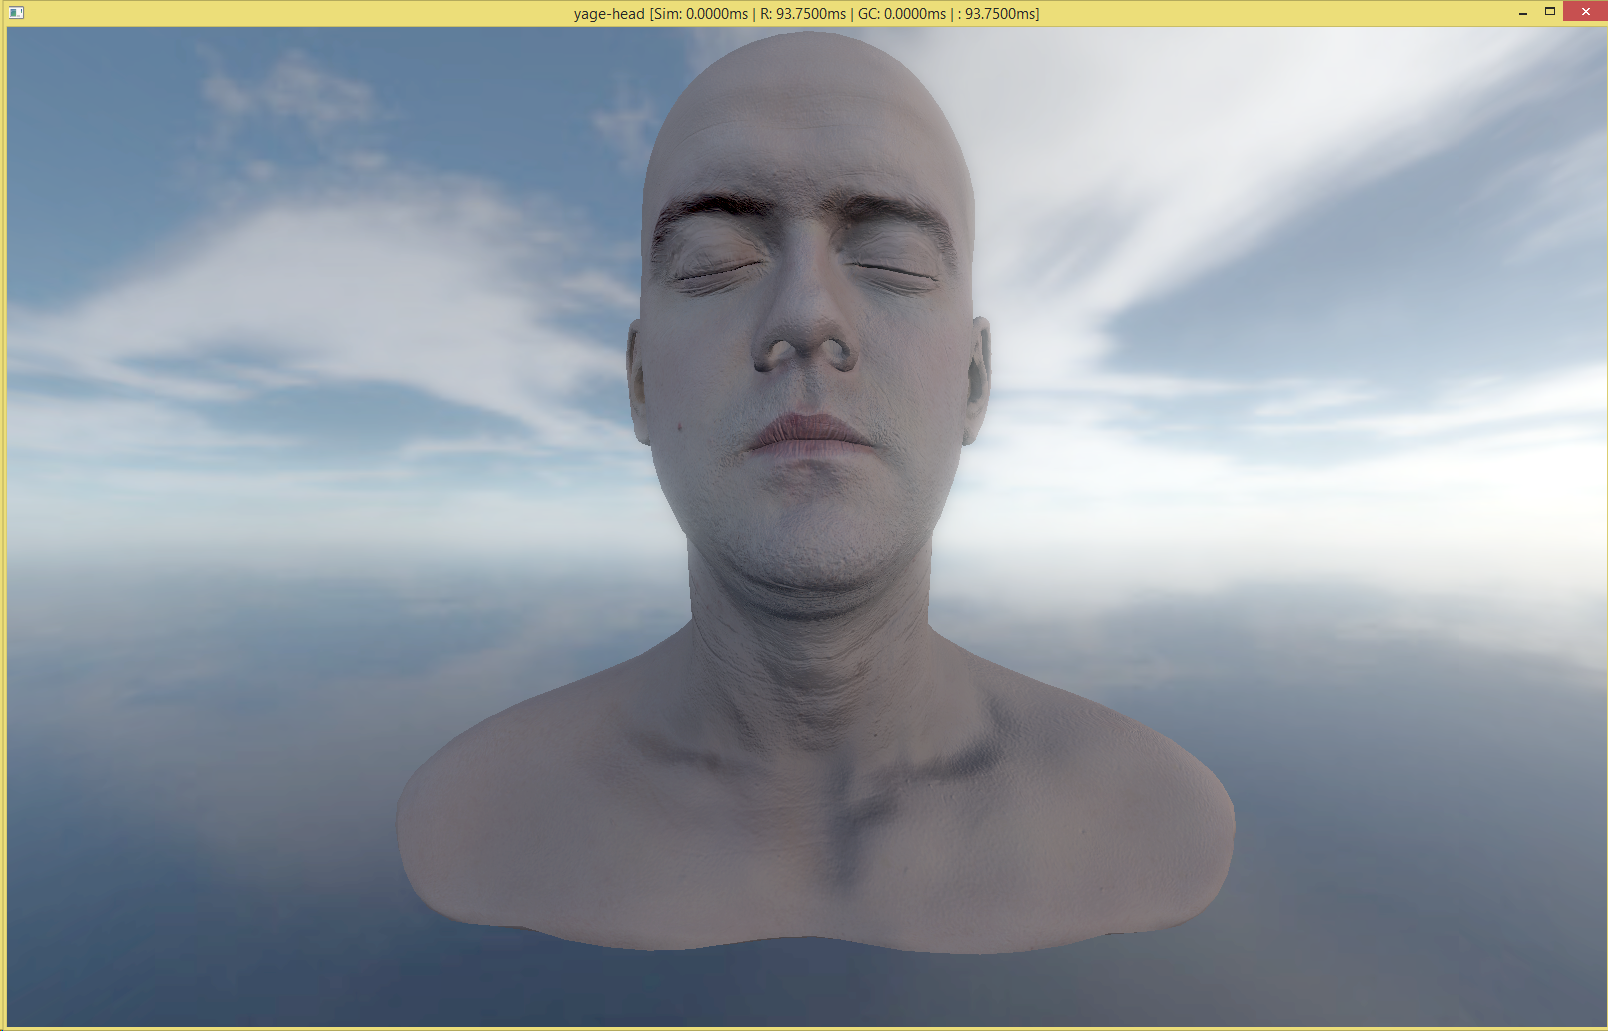
\includegraphics[width=.7\textwidth]{shots/head}
	\caption{Head}\label{fig:impl-scenes-head}
\end{subfigure}\\
\begin{subfigure}{\textwidth}
	\centering
	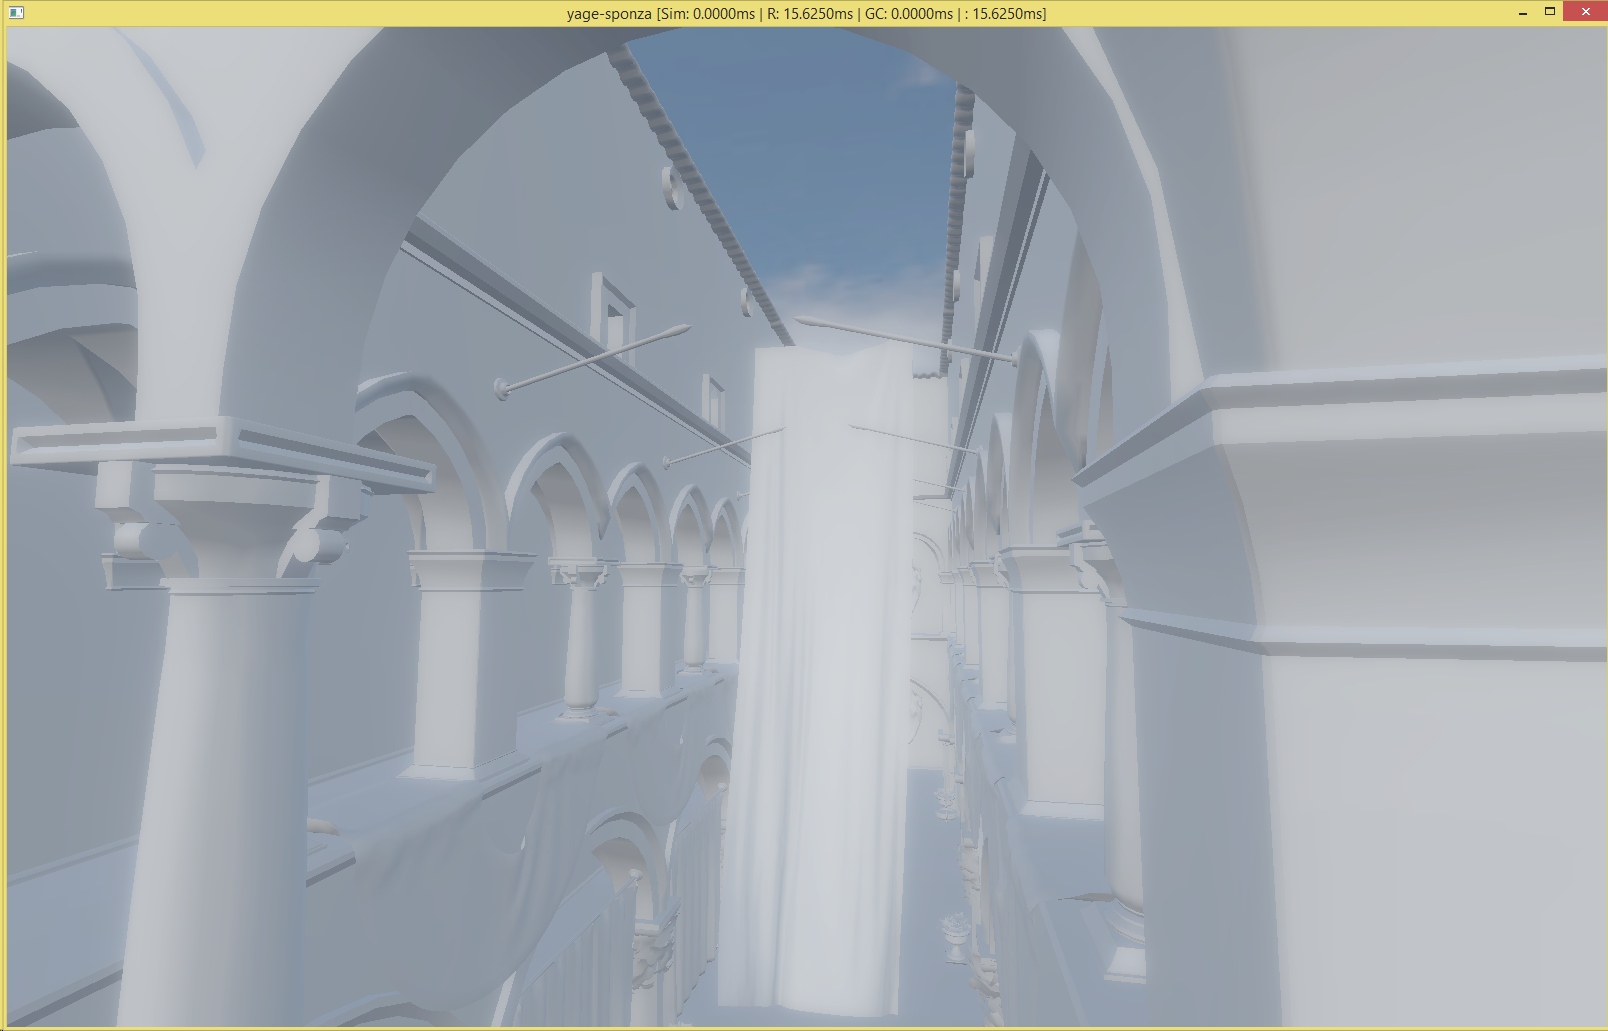
\includegraphics[width=.7\textwidth]{shots/sponza-ibl01}
	\caption{Sponza}\label{fig:impl-scenes-sponza}
\end{subfigure}\\
\begin{subfigure}{\textwidth}
	\centering
	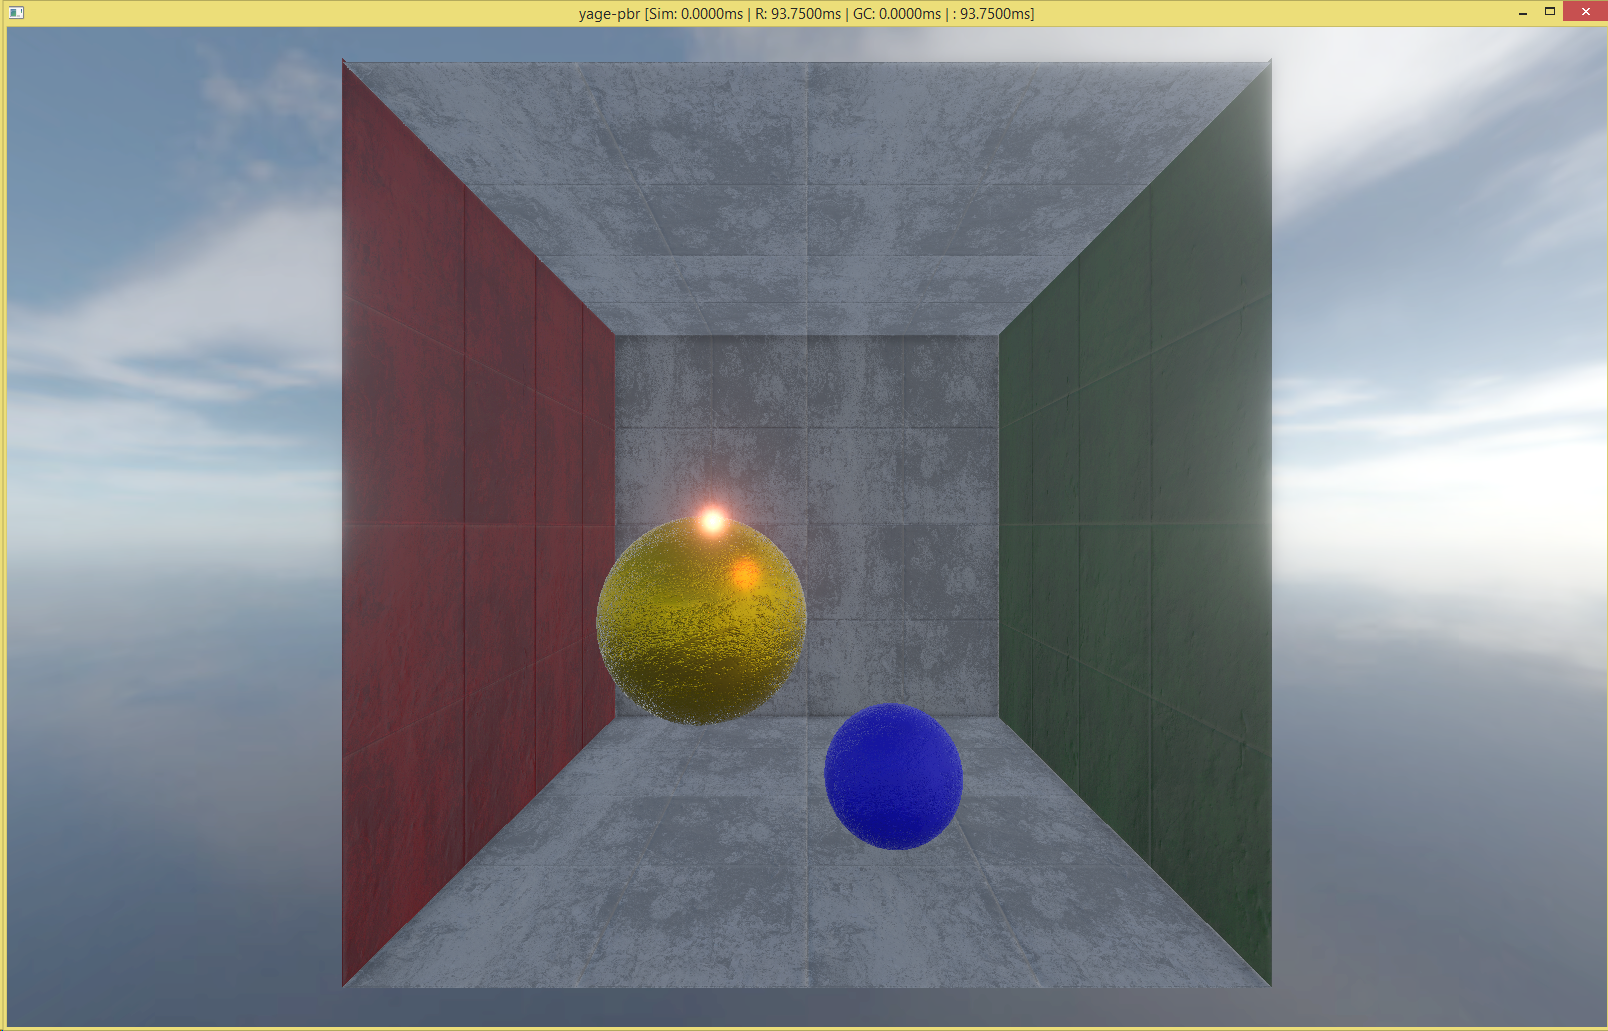
\includegraphics[width=.7\textwidth]{shots/box-blue-start}
	\caption{Box}\label{fig:impl-scenes-box}
\end{subfigure}
\caption{Implementierung Testszenen}\label{fig:impl-scenes}
\end{figure}

\subsection{Testszenen}\label{sec:testszenen-impl}

Die Testszenen besitzen keinen keinen Anspruch auf Praxisnähe, sondern dienten während der Umsetzung der Engine als Funktionstest. Die Testszene in \fref{fig:impl-scenes-head} diente als Test für das Laden von einem komplexen Modell mit realistischen Texturen. \fref{fig:impl-scenes-sponza} zeigt das Sponza-Modell\footnote{http://www.crytek.com/cryengine/cryengine3/downloads} ohne Texturen aber mit aktiviertem \ac{IBL} auf Basis der gefilterten Umgebungstextur (\fref{sec:pbr-ibl}). \fref{fig:impl-scenes-box} zeigt eine generische Szene mit Testsphären für das Testen der Beleuchtungsparamter der \ac{PBR} Pipeline.

\subsection{Laufzeitverhalten}\label{sec:laufzeit-impl}

Gemessen wurde die durchschnittliche Zeit pro Render-Frame und die prozentuale CPU Last durch das Aufrufen der \textit{OpenGL}-\ac{API}. Drei Szenen (\fref{fig:impl-scenes}) wurden mit dem Programm \textit{nVidia Nsight} ausgewertet. Die Spezifikation des Testsystems ist der \fref{tab:spec-system} zu entnehmen. Die Ergebnisse werden in \fref{tab:performance} dargestellt, jeweils mit und ohne aktiviertem \ac{AO}\footnote{Ambient Occlusion wurde im Zuge des VR Projects implementiert}.


\begin{table}[h]
\centering
\begin{tabular}{@{}lcccc@{}}
\toprule
       & CPU API (\%) & GPU (ms/F) & GPU mit \ac{AO} (ms/F) & \\ \midrule
sponza & 28  		  &  15  & 134  &  \\
head   & 31    		  &  15  & 100  &  \\
box    & 23    		  &  15  & 100  &  \\ \bottomrule
\end{tabular}
\caption{Millisekunden pro Frame für drei Beispielszenen.\\Jeweils ohne und mit Ambient Occlusion}\label{tab:performance}
\end{table}

\begin{table}[h]
\centering
\begin{tabular}{@{}llc@{}}
\toprule
CPU &  Intel(R) Core(TM) i5-3570K CPU \@ 3.40GHz  & \\
GPU &  NVIDIA GeForce GTX 570  & \\
RAM &  32 GB  & \\ \bottomrule
\end{tabular}
\caption{Testsystem}\label{tab:spec-system}
\end{table}

Bisher stand die Performance der Engine nur dann im Fokus, wenn die Performance, trotz der einfachen Szenen, zum Problem wurde. Das war in der Projektphase nur zwei Mal der Fall, aktuell bei der \ac{AO} Implementierung. Techniken zur Reduzierung der API Aufrufe, wie zum Beispiel Frustum-Culling, wurden noch nicht implementiert.

\section{Erfahrungen mit Haskell}\label{sec:xp-haskell}

In der Praxis wird Haskell nicht unvoreingenommen betrachtet. Verfechter von Sprachen wie C/C++ bringen das Argument, dass Haskell (oder eine andere Sprache) eine geringere Laufzeiteffizienz als C/C++ aufweise. Dies stimmt zwar prinzipiell, doch sind selbst in zeitkritischen Anwendungen nicht alle Komponenten gleich kritisch. Zudem hat die Wahl der geeigneten Algorithmen einen grundlegenderen Einfluss auf die Zeiteffizienz als die Wahl der Programmiersprache. Programmiersprachen sind Kommunikationmittel die an den Menschen gerichtet sind. Entsprechend sollten Programmiersprachen primär als Werkzeug für den Entwickler betrachtet werden, die Form des Problems sollte die Wahl des Werkzeugs bestimmen. In \fref{sec:engines-herausforderungen} und \fref{chap:loesungen-durch-fp} wurden aktuelle treibende Probleme in der Softwareentwicklung benannt und aufgezeigt, dass Haskell diese Probleme lösen kann oder ihnen gar nicht unterliegt, wie beispielsweise die \texttt{NULL} Problematik oder den \textit{Shared State} in nebenläufigen Anwendungen.

% \begin{figure}
% \centering
% \includegraphics[width=10cm]{benchmarkgame-chart}
% \caption{Benchmark Game: binary-trees\protect\footnotemark}\label{fig:benchmark-chart}
% \end{figure}
% \footnotetext{http://benchmarksgame.alioth.debian.org/u32/performance.php?test=binarytrees}

Die Produktivität der Entwickler sollte nicht unter allen Umständen der Laufzeiteffizient geopfert werden. Ein laufzeiteffizientes und doch gescheitertes Projekt bleibt ein gescheitertes Projekt. Der Gründer von \textit{Epic Games} (\textit{Unreal Engine}) würde 10\% der Performance für 10\% mehr Produktivität opfern \parencite[Seite 20]{Sweeney2006}.


% Next Mainstream Programming Language

\subsection{Vorteile von Haskell}

In \fref{chap:loesungen-durch-fp} wurden schon einige Vorzüge von Haskell diskutiert: Die Möglichkeit zur Abstraktion, die Kompositionsfähigkeit, die Ad-Hoc Beweisführung, das Begünstigen von Multi-Threading durch unveränderliche Daten. Haskell besitzt für viele Probleme in der Softwareentwicklung Lösungen und Lösungskonzepte. 

Abseits der genannten Vorzüge zeigt beispielsweise die Implementierung des Renderschritts in \fref{chap:anwendung}, dass Haskell zudem auch imperative Programmierung erlaubt, sollte dies punktuell notwendig sein. Die Implementierung des Renderschritts folgt in dem Beispiel der imperativen Natur der \textit{OpenGL}-\ac{API}. Hierbei zeigt sich, dass sich funktionale Konzepte gut mit imperativer Programmierung mischen lassen. Viele Konzepte aus Haskell haben inzwischen ihren Einzug in andere imperative Sprachen gefunden: Lambda-Funktionen in C++ und Java, Monaden in C\#\footnote{http://blogs.msdn.com/b/wesdyer/archive/2008/01/11/the-marvels-of-monads.aspx} oder die Strategie Objekte als unveränderlich (immutable) zu entwickeln, damit Multi-Threading sicher und einfacher umgesetzt werden kann \parencite[Seite 46ff]{Peierls:2005:JCP:1076522}.

Ein großer Vorteil von Haskell ist der \ac{GHC}, der eine sehr aktive Entwicklergemeinde besitzt\footnote{https://phabricator.haskell.org/} und fortlaufend verbessert und erweitert wird. Der \ac{GHC} ist ein herausragendes Beispiel für eine "`Real World"' Anwendung von Haskell. Im Vergleich mit dem \textit{gcc} Compiler\footnote{https://gcc.gnu.org/onlinedocs/gcc/Contributors.html} für C/C++ ist die aktive Entwicklergemeine des \ac{GHC} sehr klein\footnote{https://www.haskell.org/ghc/contributors}. C und C++ befinden sich schon jahrelang in einer breiten Anwendung und die Compiler wurden laufend weiterentwickelt und optimiert, teils mit Unterstützung großer Unternehmen wie \textit{IBM} oder \textit{Intel}. Daraus lässt sich schlussfolgern, dass große Fortschritte durch Optimierungen des Compilers nicht mehr zu erwarten sind --- `die "`low hanging fruits"' dürften schon alle gepflückt worden sein'. Haskell und der \ac{GHC} könnten noch einige Optimierungen ermöglichen (Spekulation). Zum einen begünstigt durch die Tatsache, dass viele gereifte Optimierungen aus anderen Sprachen sich nicht ohne weiteres auf Haskell anwenden lassen, und zum anderen eröffnet die Möglichkeit zur Abstraktion in Haskell neue Spielräume für den Compiler. Zum Beispiel erleichtert die referenzielle Transparenz von Haskell dem Compiler sichere Transformationen des Quelltextes\footnote{oder der Zwischensprache} zur Übersetzungszeit vorzunehmen, während in imperativen Sprachen die Neuanordnung von effektbehafteten Operationen nicht trivial ist. Und zum anderen konnten in den \ac{GHC}, aufgrund der kleineren Entwicklergemeinde, in der Summe deutlich weniger Arbeitsstunden investiert werden\footnote{http://www.quora.com/Is-Haskell-as-fast-as-C++-If-not-why-not}.

\subsection{Probleme mit Haskell}\label{sec:probleme-haskell}

Die produktive Verwendung von Haskell bringt aber auch einige Probleme mit sich. Oft sind die Probleme aber eher organisatorischer und menschlicher Natur. Zum einen sind die funktionalen Konzepte, beispielsweise im Vergleich zu den OOP Konzepten, nicht auf breiter Front bekannt und erfordern neue Denkmuster. Die bestehenden Denkmuster konnten sich jahrelang verfestigen. Deswegen stoßen neue Denkansätze auf Widerstand.

Das schrittweise Einführen (Drop In Replacement) von Haskell ist nicht immer einfach. Während sich in modernen Serverarchitekturen selektiv einige kleine isolierte Dienste mit Haskellimplementierungen ersetzen lassen, stellt sich das bei monolithischen Projekten als schwer bis unmöglich heraus. Auch ist die Verknüpfung von Haskell mit C++ noch nicht umfassend gelöst.

Zudem mangelt es Haskell an wirklich umfassenden Entwicklungsumgebungen. Zwar ist die \textit{Emacs} Unterstützung herausragend, doch fehlt es an grafischen \ac{IDE}s, die eine ähnliche Entwicklerunterstützung bieten wie zum Beispiel \textit{Eclipse} für Java oder {Visual Studio} für C++ und .Net. Das schreckt einige Entwickler ab.

Abschließend lässt sich das Fazit zeihen, dass Haskell an Vorurteilen und dem Henne-Ei Problem leidet. Durch die geringe Wahrnehmung von Haskell im produktiven Umfeld wird Haskell die Eignung neben der akademischen Anwendung abgesprochen. Viele kommerzielle Anwendungen von Haskell existieren entweder nur vorborgen oder hinter verschlossenen Türen. Beispielsweise ist es einer Webseite die verwendet Technologie nicht anzumerken\footnote{Chordify verwendet Haskell zur Akkord-Erkennung von Musik: http://chordify.net/}. Ist die Schwelle der Wahrnehmung einmal überschritten, könnten die Vorzüge von Haskell schnell überzeugen. Trotz der geringen Wahrnehmung im praktischen Umfeld, existiert eine Haskell-Gemeinde die regelmäßig Biblitheken entwickelt, die sich aktuellen technologischen Problemen widmen\footnote{reddit.com/r/haskell/}. Sind Entwickler einmal von Haskell überzeugt, scheint Haskell die Motivation zu liefern, weiter in der Sprache zu entwickeln, trotz der geringen Reichweite. Persönlich kann der Autor das bestätigen.
